\chapter[Структура кода]{Структура кода}
\label{chap:code_structure}

\section[Объектно-ориентированное программирование и данные микрогравиметрии]{Объектно-ориентированное программирование и данные микрогравиметрии}
\label{sec:object-oriented programming_and_microgravity_data}

Этот мощный способ программирования, для которого особенно подходит Python,
основан на наборе определений объектов (классов), которые содержат оба атрибута
(или свойства), такие как временной ряд, имя, словарь других объектов… и методы
(или функции/определения), которые описывают, что может делать объект. Таким
образом, этот метод программирования не является линейным, но способствует
удобочитаемости кода, как только программист привыкает к таким концепциям.
Метод, например, для записи новых выходных форматов, может быть легко добавлен в
соответствующий объект и вызван из основной программы, добавив всего несколько
строк и сохранив общий фрейм исходного кода.

Это особенно подходит для данных о микрогравитации, главным образом потому, что
данные могут быть организованы в виде структур (объектов) в соответствии с
иерархическим определением (кампания, которая включает в себя несколько опросов,
которые включают в себя несколько циклов, которые включают в себя несколько
станций, которые включают временные ряды полученных данных). Объекты могут быть
физически идентифицированы (кампания, опрос, цикл, станция), а также связанные с
ними методы (чтение ascii-файла CG5 должно быть определено в самом широком
объекте - кампании; запись входного файла mcgravi – файла ‘c’ - для
корректировки дрейфа должна быть определена в объекте цикла, в то время как
корректировка дрейфа должна вызываться или основываться на объекте съемки; выбор
данных будет в основном касаться станций). Эта логическая иерархия позволяет
хранить данные в виде структур.

\section[Графический интерфейс и PyQt]{Графический интерфейс и PyQt}
\label{sec:gui_and_pyqt}

yQt использует мощный язык программирования python и его пригодность для
объектно-ориентированного программирования вместе с библиотеками Qt GUI
(графический пользовательский интерфейс). PyQt состоит из нескольких модулей,
таких как фундаментальный QtCore (для функций, отличных от gui, таких как
использование файлов, потоков, процессов или времени) и QtGui (для графических
компонентов), среди которых определены от десятков до сотен классов, содержащих
многочисленные функции и свойства.

\section[Код pyGrav]{Код pyGrav}
\label{sec:pygrav_code}

Код основан на объектно-ориентированном программировании (ООП). Это можно
рассматривать как два параллельных набора определений:
\begin{itemize}
    \item Функции хранения данных и манипулирования ими: ядро программы, где
    определены классы и функции для операций с данными. Это тот самый
    \verb|data_object.py| исходный файл.

    \item Функции GUI: функции графического интерфейса пользователя, которые
    связывают требования пользователя с операциями с данными, определенными в
    предыдущем наборе определений. Это тот самый \verb|pyGrav_main.py| исходный
    файл.
    
\end{itemize}

В целом, код обильно прокомментирован, и описан каждый класс, подкласс, функции и свойства.

\subsection[Объектный файл данных]{Объектный файл данных}
\label{subsec:data_object_file}

Этот модуль содержит основные классы программы:
\begin{itemize}
    \item Базовый класс - это объект типа Channel List, который в основном
    содержит списки каналов, подобные тем, что содержатся в выходных файлах CG5
    ascii (сила тяжести, наклоны, температура, стандартное отклонение, время
    ...).

    Производные классы следуют логической иерархии, где каждый "подкласс"
    создается как элемент словаря из родительского класса:
    \begin{itemize}
        \item класс Campaign содержит словарь объектов типа "Опрос"
        \begin{itemize}
            \item class Survey содержит словарь объектов типа "Цикл".
            % \begin{itemize}
                \item цикл класса содержит словарь объектов типа 'Station'.
                % \begin{itemize}
                    \item станция класса o содержит временные ряды для каждой станции
                % \end{itemize}
            % \end{itemize}
        \end{itemize}
    \end{itemize}
    
\end{itemize}

Каждый из этих объектов является производным от объекта списка каналов.
Экземпляр базового класса 'Campaign' содержит весь набор данных. У каждого
класса также есть определенные свойства и функции заполнения, записи, обработки
и processing, вызываемые из основной программы (рис. 1).

\begin{figure}
    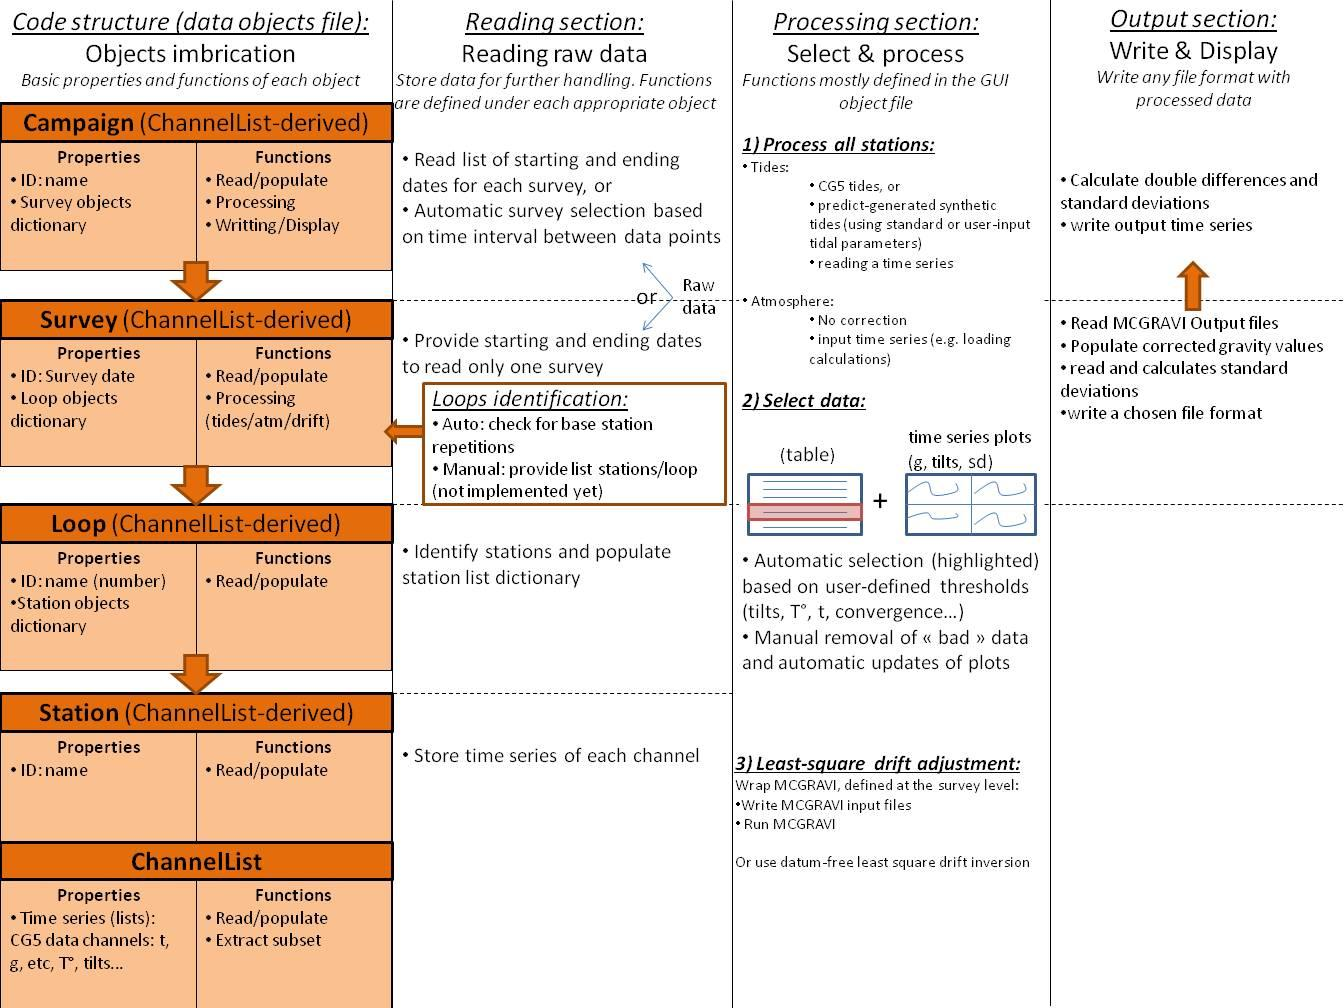
\includegraphics[width=\textwidth]{figures/pygrav_chart_and_structures_imbrications}
    \caption{Диаграмма pyGrav и обозначения структур (объектов) : в объекте
    кампании есть словарь из нескольких опросов. В объекте обзора есть словарь
    из нескольких циклов. В объекте цикла есть словарь из нескольких станций.
    Каждый из этих объектов является производным от объекта Channel List (т.е.
    они содержат несколько временных рядов).}
    \label{fig:pygrav_chart_and_structures_imbrications}
\end{figure}

\subsection[Файл графического интерфейса]{Файл графического интерфейса}
\label{subsec:gui_file}

Это файл, который должен быть выполнен для запуска pyGrav. Он содержит
единственный класс под названием main Prog, который является объектом
QMainWindow, производным от Qt. Наиболее важными свойствами класса mainProg
являются объект Campaign, который содержит весь набор данных, а также каталоги
данных и выходных данных. Большинство функций класса mainProg связывают
пользовательский интерфейс (определенный в функциях) с кодом обработки,
записанным в файле объекта данных, для изменения состояний объекта Campaign
(набора данных).

\section*{Ссылки}

Несколько ссылок для тех, кто заинтересован в изменении кода

Несколько руководств по Python:

\url{https://docs.python.org/2/tutorial/} Руководство для Python версии 2.7

\url{http://zetcode.com/lang/python/}

\url{http://marvin.cs.uidaho.edu/Teaching/CS515/pythonTutorial.pdf} (Руководство G. Van Rossum)

Руководство PyQt:

\url{http://zetcode.com/gui/pyqt4/}

Ссылки на класс PyQt:

\url{http://pyqt.sourceforge.net/Docs/PyQt4/classes.html}

Демо графиков PyQt:

\url{http://eli.thegreenplace.net/2009/05/23/more-pyqt-plotting-demos/}

Руководства программирования вида модели:

\url{http://www.yasinuludag.com/blog/?p=98}

Руководство Matplotlib:

\url{http://web.archive.org/web/20100830233506/http://matplotlib.sourceforge.net/leftwich_tut.txt}